\tikzset{every picture/.style={line width=0.75pt}}

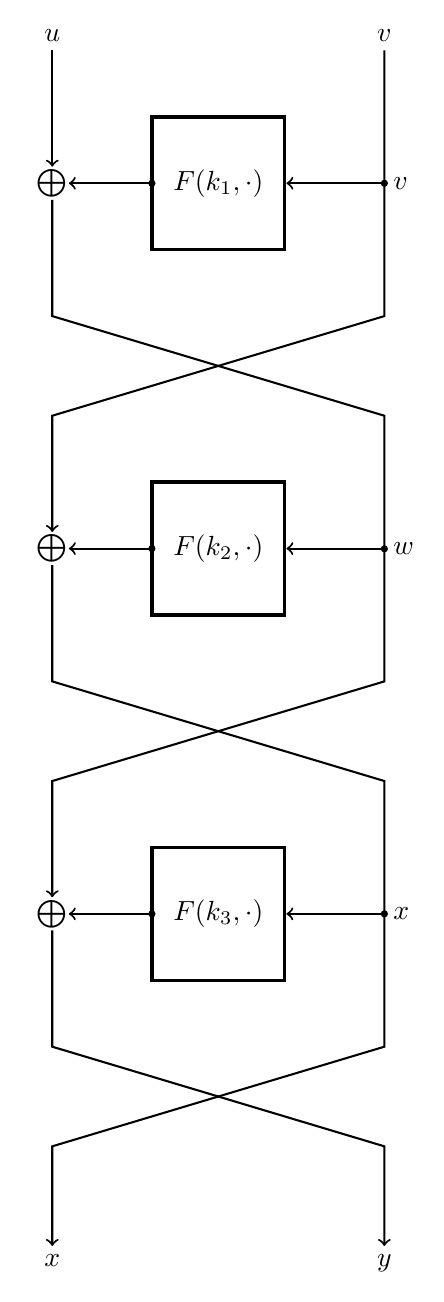
\begin{tikzpicture}[x=0.75pt,y=0.75pt,yscale=-0.8,xscale=0.8]


\draw  [line width=1.2]  (80,80) -- (160,80) -- (160,160) -- (80,160) -- cycle ;
\draw  [line width=1.2]  (80,300) -- (160,300) -- (160,380) -- (80,380) -- cycle ;
\draw  [line width=1.2]  (80,520) -- (160,520) -- (160,600) -- (80,600) -- cycle ;

\draw  [->]  (20,40) -- (20,110) ;
\draw  [->]  (20,130) -- (20,200) -- (220,260) -- (220,420) -- (20,480) -- (20,550) ;
\draw  [->]  (20,570) -- (20,640) -- (220,700) -- (220,760) ;
\draw  [->]  (220,40) -- (220,200) -- (20,260) -- (20,330) ;
\draw  [->]  (20,350) -- (20,420) -- (220,480) -- (220,640) -- (20,700) -- (20,760) ;

\draw  [->]  (80,120) -- (30,120) ;
\draw  [->]  (220,120) -- (161,120) ;
\draw  [->]  (80,340) -- (30,340) ;
\draw  [->]  (220,340) -- (161,340) ;
\draw  [->]  (80,560) -- (30,560) ;
\draw  [->]  (220,560) -- (161,560) ;

\draw  [fill={rgb, 255:red, 0; green, 0; blue, 0 }  ,fill opacity=1 ] (218.5,120) .. controls (218.5,119.17) and (219.17,118.5) .. (220,118.5) .. controls (220.83,118.5) and (221.5,119.17) .. (221.5,120) .. controls (221.5,120.83) and (220.83,121.5) .. (220,121.5) .. controls (219.17,121.5) and (218.5,120.83) .. (218.5,120) -- cycle ;
\draw  [fill={rgb, 255:red, 0; green, 0; blue, 0 }  ,fill opacity=1 ] (78.5,120) .. controls (78.5,119.17) and (79.17,118.5) .. (80,118.5) .. controls (80.83,118.5) and (81.5,119.17) .. (81.5,120) .. controls (81.5,120.83) and (80.83,121.5) .. (80,121.5) .. controls (79.17,121.5) and (78.5,120.83) .. (78.5,120) -- cycle ;
\draw  [fill={rgb, 255:red, 0; green, 0; blue, 0 }  ,fill opacity=1 ] (78.5,340) .. controls (78.5,339.17) and (79.17,338.5) .. (80,338.5) .. controls (80.83,338.5) and (81.5,339.17) .. (81.5,340) .. controls (81.5,340.83) and (80.83,341.5) .. (80,341.5) .. controls (79.17,341.5) and (78.5,340.83) .. (78.5,340) -- cycle ;
\draw  [fill={rgb, 255:red, 0; green, 0; blue, 0 }  ,fill opacity=1 ] (218.5,340.15) .. controls (218.5,339.33) and (219.17,338.65) .. (220,338.65) .. controls (220.83,338.65) and (221.5,339.33) .. (221.5,340.15) .. controls (221.5,340.98) and (220.83,341.65) .. (220,341.65) .. controls (219.17,341.65) and (218.5,340.98) .. (218.5,340.15) -- cycle ;
\draw  [fill={rgb, 255:red, 0; green, 0; blue, 0 }  ,fill opacity=1 ] (218.5,560) .. controls (218.5,559.17) and (219.17,558.5) .. (220,558.5) .. controls (220.83,558.5) and (221.5,559.17) .. (221.5,560) .. controls (221.5,560.83) and (220.83,561.5) .. (220,561.5) .. controls (219.17,561.5) and (218.5,560.83) .. (218.5,560) -- cycle ;
\draw  [fill={rgb, 255:red, 0; green, 0; blue, 0 }  ,fill opacity=1 ] (78.5,560) .. controls (78.5,559.17) and (79.17,558.5) .. (80,558.5) .. controls (80.83,558.5) and (81.5,559.17) .. (81.5,560) .. controls (81.5,560.83) and (80.83,561.5) .. (80,561.5) .. controls (79.17,561.5) and (78.5,560.83) .. (78.5,560) -- cycle ;

\draw (20,120) node  [font=\large]  {$\bigoplus $};
\draw (20,340) node  [font=\large]  {$\bigoplus $};
\draw (20,560) node  [font=\large]  {$\bigoplus $};
\draw (120,120) node    {$F( k_{1} ,\cdot )$};
\draw (120,340) node    {$F( k_{2} ,\cdot )$};
\draw (120,560) node    {$F( k_{3} ,\cdot )$};
\draw (20,36.6) node [anchor=south] [inner sep=0.75pt]    {$u$};
\draw (220,36.6) node [anchor=south] [inner sep=0.75pt]    {$v$};
\draw (223.5,120) node [anchor=west] [inner sep=0.75pt]    {$v$};
\draw (223.5,340.15) node [anchor=west] [inner sep=0.75pt]    {$w$};
\draw (223.5,560) node [anchor=west] [inner sep=0.75pt]    {$x$};
\draw (20,763.4) node [anchor=north] [inner sep=0.75pt]    {$x$};
\draw (220,763.4) node [anchor=north] [inner sep=0.75pt]    {$y$};


\end{tikzpicture}